\documentclass[11pt]{article}
\usepackage{amsmath,amssymb,amsthm,mathtools}
\usepackage{iftex}
\ifPDFTeX
  \usepackage[T1]{fontenc}
\else
  \usepackage{unicode-math}
  \setmainfont{STIX Two Text}
  \setmathfont{STIX Two Math}
  \setmonofont{DejaVu Sans Mono}[Scale=MatchLowercase]
\fi
\usepackage[margin=1in]{geometry}
\usepackage{booktabs,array,longtable}
\usepackage{microtype}
\usepackage{xurl}
\emergencystretch=3em
\usepackage{hyperref}
\hypersetup{hidelinks,pdftitle={Classical consistency and quantum purification without a fixed causal order},pdfauthor={Drew Lamarr Arrowood}}
\usepackage{tikz}
\usetikzlibrary{arrows.meta,positioning}

\newtheorem{theorem}{Theorem}
\newtheorem{lemma}[theorem]{Lemma}
\newtheorem{corollary}[theorem]{Corollary}
\newtheorem{proposition}[theorem]{Proposition}
\theoremstyle{definition}
\newtheorem{definition}[theorem]{Definition}
\theoremstyle{remark}
\newtheorem{remark}[theorem]{Remark}

\newcommand{\ket}[1]{\lvert #1\rangle}
\newcommand{\bra}[1]{\langle #1\rvert}
\newcommand{\conv}{\operatorname{conv}}
\newcommand{\PF}{\mathrm{PF}}
\newcommand{\Purif}{\mathrm{Purif}}
\newcommand{\Valid}{\mathrm{Valid}}

\title{Classical consistency and quantum purification\\ without a fixed causal order}
\author{Drew Lamarr Arrowood\thanks{Affiliation and correspondence address: pending confirmation by the author. ORCID: not recorded in the source manuscript. This file is a draft for the author's review. It has not been submitted.}}
\date{Draft, 7 November 2026}

\begin{document}
\maketitle

\begin{abstract}
Local laboratories that may choose any operation, with no assumed order among them, still have to return probabilities. For deterministic classical processes this demand is exact: every choice of local functions must have exactly one consistent history. Such processes are process functions. Adding a source and a sink turns every process function into a permutation, but a permutation of a basis is not yet a quantum process. We prove that the canonical reversible extension, composed with arbitrary local unitaries and finite ancillas, induces a unitary from source to sink, and that this happens for every choice of those unitaries if and only if the classical map is a process function. Stinespring dilation then yields validity under arbitrary local instruments. Mixtures of process functions arise by recording a coherent label in the sink, so they are purifiable. The converse fails. An explicit three-party binary machine, unitary under every local unitary, induces in the computational basis a valid classical process that violates a linear inequality satisfied by every process function, with value \(\tfrac14-\tfrac{3}{16}\sqrt{2}<0\). Quantum purification is therefore strictly weaker than being a mixture of deterministic consistent processes. The argument is not a spacetime realisation, and it does not decide which further classical processes are purifiable.
\end{abstract}

\noindent\textbf{Keywords.} process function; indefinite causal order; unitary process; purification; process matrix

\section{Introduction: consistency versus purification}
\label{sec:intro}

A process matrix assigns a probability to every choice of local instruments, without assuming a global causal order among the laboratories \cite{oreshkov2012,araujo2017}. The deterministic classical points of that theory are process functions: maps from the parties' outputs to their inputs such that every tuple of local functions has exactly one fixed point \cite{baumeler2016,baumeler2019}. The fixed-point clause does two jobs at once. No fixed point is a history that contradicts itself. More than one fixed point is a history the local choices do not determine. The parties are not forbidden any local operation; only the global solution is constrained \cite{baumeler2019}.

Two questions follow. First, does every such deterministic consistent process extend to a unitary quantum process? Baumeler, Costa, Ralph, Wolf and Zych showed that a source and a sink turn every process function into a bijection, and left open whether that bijection quantises \cite{baumeler2019}. Special cases were settled later: the Lugano process \cite{araujo2017}, an \(n\)-party family \cite{araujo2017b}, and unitaries with mutually exclusive control conditions \cite{daher2026}. The general finite-alphabet statement was formulated as a conjecture by Daher Ahmed and Kunjwal \cite{daher2026}. Theorem~\ref{thm:lift} below is a proof for every process function on finite alphabets, and Theorem~\ref{thm:iff} is the converse: unitarity for every local unitary holds only for process functions.

Second, does quantum purification recover only mixtures of those deterministic processes? Mixtures do purify, by a coherent label kept at the sink. The converse was a natural conjecture and is false. Theorem~\ref{thm:sep} gives a valid three-party binary classical process, induced by an explicit pure process in the computational basis, that lies outside the convex hull of the process functions. The numerical value of the separating inequality is \(\tfrac14-\tfrac{3}{16}\sqrt{2}\). The same process is known, up to a local frame, as a time-reversed variant of a Lugano purification \cite{guerin2018,baumeler2019}; what is separated here is the classical process it induces in a stated basis, not the existence of the quantum board.

The article is organised as follows. Section~\ref{sec:def} fixes the finite operational setting. Section~\ref{sec:lift} proves the lift and its converse, and records the passage from unitarity to validity. Section~\ref{sec:pur} constructs the separation. Section~\ref{sec:bounds} states what the two theorems do and do not say about causal order, two parties, and spacetime. Section~\ref{sec:disc} lists the open problems that remain inside this formalism. A short derivation of validity, the witness tables, and a note on formal verification are in the appendices. The public technical archive \cite{archive} contains the proofs, the machine-checked formalisation, and a large body of material deliberately omitted here.

\section{Operational setting and definitions}
\label{sec:def}

Throughout the main theorems there are finitely many parties \(k\in\{1,\ldots,n\}\), each with a finite nonempty input alphabet \(I_k\) and a finite nonempty output alphabet \(O_k\). For the permutation form of the lift we identify \(I_k\) with the cyclic group \(\mathbb{Z}_{|I_k|}\). The product spaces are written \(O=\prod_k O_k\) and \(I=\prod_k I_k\).

\begin{definition}[Process function]
\label{def:pf}
A map \(w=(w_k):O\to I\) is a \emph{process function} when, for every tuple of local functions \(f_k:I_k\to O_k\), the self-map of \(O\) given by
\[
o\;\longmapsto\;\bigl(f_k(w_k(o))\bigr)_k
\]
has exactly one fixed point.
\end{definition}

A fixed point is a consistent history for that intervention. The quantifier ranges over every local function, including those that are not causal functions of a background time. Acyclic deterministic circuits are process functions, but they are not all of them. The three-bit Lugano map
\begin{equation}
\label{eq:lugano}
w(a,b,c)=(\lnot b\land c,\;\lnot c\land a,\;\lnot a\land b)
\end{equation}
has a cyclic dependence and exactly one fixed point for every choice of local bit functions \cite{baumeler2016,araujo2017}. For two binary parties the twelve process functions are all causally ordered \cite{oreshkov2012,baumann2016}.

The reversible extension uses a source, whose output space we identify with \(I\), and a sink, whose input space we identify with \(O\). For a basis vector \(\ket{o}\) of the output registers and a basis vector \(\ket{e}\) of the source,
\begin{equation}
\label{eq:U}
U\ket{o}_O\ket{e}_P=\ket{w(o)+e}_I\ket{o}_F,
\end{equation}
with addition in each \(I_k\). For every function \(w\), not only for process functions, \(U\) is a permutation of a finite basis and hence unitary \cite{baumeler2019}. Unitarity of \(U\) alone is not the quantum condition. Each party may insert a unitary that is not diagonal in the chosen basis, with a private ancilla.

\begin{definition}[Closed loop]
\label{def:loop}
Let \(V_k\) be a unitary from \(I_k\otimes X_k\) to \(O_k\otimes Y_k\), with finite ancilla spaces satisfying \(|I_k|\,|X_k|=|O_k|\,|Y_k|\). Wiring each input factor of \(U\) into \(V_k\) and each output factor of \(V_k\) back into \(U\) defines an operator \(M\) from \(P\otimes X\) to \(F\otimes Y\), \(X=\bigotimes_k X_k\) and \(Y=\bigotimes_k Y_k\), with matrix elements
\begin{equation}
\label{eq:M}
M\bigl[(s,y),(e,x)\bigr]
=\prod_k V_k\bigl[(s_k,y_k),\,(w_k(s)+e_k,x_k)\bigr].
\end{equation}
\end{definition}

A process is \emph{pure} in the sense of Ara\'ujo, Feix, Navascu\'es and Brukner when every such closed loop, for every choice of local unitaries and finite ancillas, is unitary \cite{araujo2017}. Purity is stronger than the existence of one unitary dilation. A classical process is \emph{purifiable}, written \(p\in\Purif\), when it arises from a pure process by preparing a source state, measuring each party in a stated orthonormal frame, and discarding the sink. Unless a frame is named, the frame is the computational basis. The same pure process can induce a mixture of process functions in one frame and a process outside that mixture in another \cite{archive}; statements below name the frame. We write \(\PF\) for the set of process functions, \(\conv(\PF)\) for its convex hull, and \(\Valid\) for the convex set of classical processes that assign total probability one under every product of local stochastic maps \cite{baumeler2016}.

\section{The unitary lifting theorem}
\label{sec:lift}

The obstruction to unitarity of \(M\) is not bijectivity of \(U\). It is whether distinct rows of \(M\) are orthogonal after the local unitaries have been inserted. The combinatorial fact that supplies the orthogonality is pairwise exclusivity.

\begin{lemma}[Exclusivity]
\label{lem:ex}
If \(w\) is a process function and \(s\neq s'\) in \(O\), some party \(k\) has \(s_k\neq s'_k\) and \(w_k(s)=w_k(s')\).
\end{lemma}

\begin{proof}
Otherwise \(w_k(s)=w_k(s')\) implies \(s_k=s'_k\) for every \(k\). Define \(f_k(x)=s_k\) if \(x=w_k(s)\) and \(f_k(x)=s'_k\) if \(x=w_k(s')\), and define \(f_k\) arbitrarily elsewhere. The two clauses agree wherever the inputs agree. Then \(s\) and \(s'\) are distinct fixed points of one intervention.
\end{proof}

The same pairing, read without quantifying over interventions, is the consistency criterion of Dourdent, Leitherer, Boghiu, Simonov, Kunjwal and Ac\'in \cite{dourdent2026}. For finitely many parties and nonempty finite alphabets, exclusivity is equivalent to Definition~\ref{def:pf}. Uniqueness of a fixed point is the easy half: two fixed points of one intervention would be a pair with no exclusivity witness. Existence is an induction on the set of active parties, the others frozen at a background value. Adding party \(n\), the configurations already fixed on the previous parties, for two different values of party \(n\), cannot take their exclusivity witness among the frozen parties or among the parties already fixed, so the witness is party \(n\) itself, and the value \(f_n\) returns is independent of the trial value. That common value closes the loop. The induction is written out in the archive. The argument below uses only Lemma~\ref{lem:ex}, which is the half that orthogonality needs.

A single intervention shows what the definition asks for in the Lugano example \eqref{eq:lugano}. Let every party return its input unchanged. A fixed point then satisfies
\[
a=\lnot b\land c,\qquad b=\lnot c\land a,\qquad c=\lnot a\land b.
\]
If \(a=1\), then \(b=0\) and \(c=1\), but the third equation becomes \(c=0\). If \(a=0\), then \(b=0\) and \(c=0\), and \((0,0,0)\) satisfies all three equations. Exactly one history. The same count for every other triple of local bit functions is the content of ``\(w\) is a process function''; it is finite and has been enumerated. The dependence is cyclic, so the example is not an acyclic circuit relabelled.

\begin{theorem}[Unitary lift]
\label{thm:lift}
If \(w\) is a process function, then for every choice of local unitaries \(V_k\) and finite ancillas as in Definition~\ref{def:loop}, the closed loop \(M\) is unitary.
\end{theorem}

\begin{proof}
The product in \eqref{eq:M} factorises the Gram matrix. For rows \((s,y)\) and \((s',y')\),
\begin{equation}
\label{eq:gram}
\bigl(MM^{\dagger}\bigr)\bigl[(s,y),(s',y')\bigr]
=\prod_k\sum_{e_k,x_k}
V_k\bigl[(s_k,y_k),(w_k(s)+e_k,x_k)\bigr]\,
\overline{V_k\bigl[(s'_k,y'_k),(w_k(s')+e_k,x_k)\bigr]}.
\end{equation}
If \(w_k(s)=w_k(s')\), the change of variables \(i=w_k(s)+e_k\) makes the \(k\)-th factor the inner product of two rows of the unitary \(V_k\). If \(s=s'\), every factor is of this kind and the product is \(\delta_{y,y'}\). If \(s\neq s'\), Lemma~\ref{lem:ex} supplies a party with equal inputs and unequal outputs, and that factor vanishes. Thus \(MM^{\dagger}=1\). The dimension hypothesis makes \(M\) square, so \(M\) is unitary.
\end{proof}

Column norms are not a substitute for this argument: unit-norm columns need not be orthogonal. The dimension count is the only place the ancilla sizes enter the proof of Theorem~\ref{thm:lift}. Figure~\ref{fig:lift} is the wiring.

Bare bijectivity of \(U\) does not answer the quantum question. Equation~\eqref{eq:U} is a permutation for every \(w\), consistent or not. The parties are allowed to insert instruments that are not diagonal in the computational basis. A Hadamard on one wire is the simplest such instrument: it mixes the two basis states that the classical theory treated as distinct. If, after that insertion, the map from source to sink fails to be unitary, the classical fixed-point clause has not lifted, and quantum theory would be imposing an extra filter. Theorem~\ref{thm:lift} says that for a process function the filter is already in place. The rows of \(M\) are orthogonal because exclusivity, not because \(U\) is a permutation. Daher Ahmed and Kunjwal note that the bare permutation may fail to be a valid process and prove the lift for unitaries with mutually exclusive control conditions \cite{daher2026}. The factorisation \eqref{eq:gram} is the general case: the control conditions need not be exclusive in their sense, because the local unitaries are arbitrary and the cancellation is supplied by Lemma~\ref{lem:ex}.

The same identity explains the ancilla quantifiers. Each \(V_k\) is an arbitrary unitary between the input leg tensored with a private ancilla and the output leg tensored with a private ancilla, provided the two legs have equal finite dimension so that a unitary between them can exist. The ancillas may be entangled with each other and with the source in the incoming state. The theorem does not quantify over a single fixed ancilla dimension. It quantifies over all finite dimensions and all unitaries of those dimensions. Shared entanglement is an incoming state, not an extra hypothesis.

\begin{figure}[t]
\centering
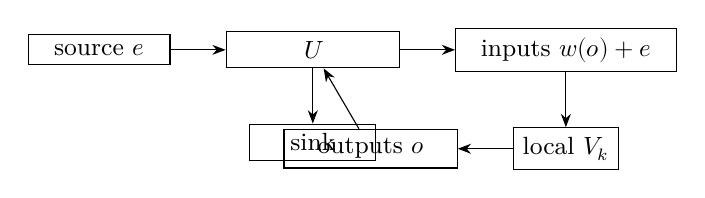
\begin{tikzpicture}[font=\small,>=Stealth,node distance=7mm]
  \node[draw,minimum width=18mm] (P) {source \(e\)};
  \node[draw,right=of P,minimum width=22mm] (U) {\(U\)};
  \node[draw,right=of U,minimum width=28mm] (I) {inputs \(w(o)+e\)};
  \node[draw,below=of I] (V) {local \(V_k\)};
  \node[draw,left=of V,minimum width=22mm] (O) {outputs \(o\)};
  \node[draw,below=of U,minimum width=16mm] (F) {sink};
  \draw[->] (P) -- (U);
  \draw[->] (O) -- (U);
  \draw[->] (U) -- (I);
  \draw[->] (I) -- (V);
  \draw[->] (V) -- (O);
  \draw[->] (U) -- (F);
\end{tikzpicture}
\caption{The reversible extension \(U\) and one local unitary. The sink records the output string. The source records the difference between the input and \(w(o)\).}
\label{fig:lift}
\end{figure}

\begin{theorem}[Unitarity for every local unitary characterises process functions]
\label{thm:iff}
Let \(w:O\to I\) be any map between finite alphabets, with each \(I_k\) a cyclic group as above. The closed loop \(M\) is unitary for every choice of local unitaries and finite ancillas if and only if \(w\) is a process function.
\end{theorem}

\begin{proof}
The direction from a process function to unitarity is Theorem~\ref{thm:lift}. Conversely, suppose some intervention \(f=(f_k)\) has \(N\neq 1\) fixed points, where \(N=0\) and \(N\ge 2\) are both allowed. Take ancillas \(X_k=O_k\) and \(Y_k=I_k\), and
\[
V_k\ket{i,x}=\ket{f_k(i)+x,\,i},
\]
addition in \(O_k\). This is a permutation of basis states, hence unitary. The entries of column \((0,0)\) of \(M\) are
\[
M\bigl[(s,y),(0,0)\bigr]
=\prod_k [s_k=f_k(w_k(s))]\,[y_k=w_k(s)],
\]
so the squared norm of that column equals the number of fixed points of \(f\). That number is not \(1\), and \(M\) is not an isometry.
\end{proof}

The gadget uses \(|I_k|\,|O_k|=|O_k|\,|I_k|\) and does not require \(|I_k|=|O_k|\). The same column, read at a general ancilla index \((e,x)\), counts the fixed points of the shifted intervention \(i\mapsto f(i+e)+x\). One failing test is enough for the converse. The forward direction demands that every test pass. The two directions are not the same theorem: orthogonality of rows uses exclusivity, while the column norm uses a specially chosen unitary to count solutions. A map can have unit columns for some interventions and fail orthogonality for others. Theorem~\ref{thm:iff} is the statement that the whole family of tests passes if and only if every intervention has exactly one fixed point.

The inverse of \eqref{eq:U} is as explicit as \(U\). The sink holds the output string \(o\). The source, read backwards, holds the difference between the input and \(w(o)\). So the classical inverse is a function of the sink and the source, not a function of the output alphabet alone. This is why a process function that is not bijective on its own alphabet, the Lugano function is two-to-one on some slices, can still have a unitary dilation. Reversibility is restored by the source and the sink, not by forcing \(w\) itself to be a permutation \cite{baumeler2019}.

Purity is unitarity under local unitaries. Validity is the trace-preserving completely positive condition under arbitrary local instruments, including instruments that share ancillas with an outside system. The passage is Stinespring's dilation and does not use any further property of \(w\).

\begin{lemma}[From purity to validity]
\label{lem:valid}
If \(M\) is unitary whenever every local map is a unitary on a finite ancilla of matching dimension, then the induced process is valid under every tuple of local instruments.
\end{lemma}

\begin{proof}
A local completely positive trace-preserving map dilates to an isometry into an output space tensored with an environment \cite{stinespring1955}. Pad the input with a junk factor and the output with a complementary factor so that the two sides have equal finite dimension, and extend the isometry to a unitary by completing orthonormal bases. Theorem~\ref{thm:lift} supplies a unitary on the enlarged loop. The environments are prepared in a fixed state and then discarded. Partial trace and a fixed ancilla state preserve the trace and complete positivity, and the link product is multilinear, so the original instruments yield a trace-preserving completely positive map from the source to the sink. An instrument is a family of such maps. The same identity, applied to the Choi operator of \(U\), is the process-matrix normalisation \(\operatorname{Tr} W=1\) on the accepted local maps \cite{araujo2017,choi1975}.
\end{proof}

The finite-dimensional argument is machine-checked in the archive, including instruments and shared ancillas. Extending the alphabets from finite to arbitrary discrete sets replaces the matrix calculation by an \(\ell^2\) argument; that extension is in the archive and is not needed here. Continuous alphabets are a different problem, because a single history is typically a null set, and they are only partly treated in the archive.

One example is enough to see that the lift is not confined to causal order. The Lugano function \eqref{eq:lugano} is a process function, so Theorem~\ref{thm:lift} supplies a unitary process. Its dependence graph is a cycle. The dilation does not remove the cycle. It realises the cycle as a unitary from a source to a sink.

\section{Quantum purification exceeds deterministic mixtures}
\label{sec:pur}

A mixture of process functions is purifiable. If \(w^{(j)}\) has weight \(\lambda_j\), prepare a control register in \(\sum_j\sqrt{\lambda_j}\ket{j}\) and route the control unchanged to the sink, while the system register carries the reversible extension of \(w^{(j)}\) controlled on \(j\). The closed loop is block diagonal in the control basis with unitary blocks, hence unitary. Discarding the sink and reading the computational basis leaves the classical mixture. The same block-diagonal sum shows that \(\Purif\) is convex. This is the coherent form of an inclusion that had been asserted for the dephased process matrix \cite{baumeler2022}. The argument just given is for the coherent operator.

The converse, that nothing else is purifiable, was a conjecture of the technical archive. It is false.

\begin{theorem}[A purifiable classical process outside the process-function hull]
\label{thm:sep}
There exists a valid classical process \(p\) on three binary parties, induced in the computational basis by a pure process with a finite source, such that
\begin{equation}
\label{eq:L}
L(p)=\frac14-\frac{3}{16}\sqrt{2}<0,
\end{equation}
while \(L\ge 0\) on every process function and hence on \(\conv(\PF)\). In particular \(\conv(\PF)\subsetneq\Purif\).
\end{theorem}

The witness is a switchboard. For each output string \(o\in\{0,1\}^3\) there is a unitary \(U_o\) on \((\mathbb{C}^2)^{\otimes 3}\). Let \(H\) be the three-qubit Hadamard and let \(m_o(z)\in\{0,1,2,3\}\) be the exponents in Appendix~\ref{app:witness}, indexed by \(z\in\{0,1\}^3\) in binary order. Set
\begin{equation}
\label{eq:Uo}
U_o=H\,\mathrm{diag}\bigl(i^{m_o(z)}\bigr)\,H,
\end{equation}
so \(U_o\) is diagonal in the Hadamard basis. The pure vector is
\begin{equation}
\label{eq:V}
V\ket{o,s,t}
=\sum_e U_o[e,s]\,\ket{e}_I\ket{o}_F\ket{e\oplus t}_F.
\end{equation}
The source state is \(\phi\otimes\ket{0}\), with
\begin{equation}
\label{eq:phi}
\phi=\frac{\ket{011}+e^{-i\pi/4}\ket{100}}{\sqrt{2}},
\end{equation}
and the classical process is the computational-basis conditional distribution \(p(i\mid o)=\lvert\bra{i}U_o\phi\rvert^2\).

Three facts have to be checked, and they have different proofs.

First, \(p\) is a valid classical process: it is nonnegative, and every product of local stochastic maps has total probability one. For deterministic local functions this is a finite sum, sixty-four of them, one for each triple of functions from a bit to a bit. The sum is multilinear in the three local operations. Every stochastic local map is a convex combination of deterministic ones, so a multilinear identity that holds on the deterministic vertices holds for every product of stochastic maps. The entries of \(p\) lie in \(\mathbb{Q}(\sqrt{2})\) and each column sums to one. Both the direct expansion and an independent re-derivation from the definition of \(V\) confirm the identity in exact arithmetic; the archive records the scripts. Floating-point circuit simulations reproduce the same table to roundoff and are checks, not proofs.

Second, \(V\) is pure. The mechanism is the same exclusivity that appeared in Lemma~\ref{lem:ex}, now for a sum of basis permutations rather than for one. Compare the boards \(U_o\) and \(U_{o'}\) for two different output strings. Their mismatch is the unitary \(K=U_o U_{o'}^{\dagger}\). Expanded in the Pauli basis of three qubits, every term that appears with a nonzero coefficient must act as the identity on at least one party whose output bit differs between \(o\) and \(o'\). A single process function has a mismatch that is one Pauli string, and the condition reduces to Lemma~\ref{lem:ex}. A switchboard may superpose several such strings, each leaving a different party alone. For the exponents in Table~\ref{tab:m} that cancellation is an identity in the cyclotomic field \(\mathbb{Q}(\zeta_8)\): every forbidden coefficient is zero. There are \(2232\) of them, a finite exact check, not a sample.

That Pauli condition is the no-ancilla half of purity. Ancillas can only enlarge the set of parties whose local data differ between two rows, and a signed sum over a larger set of bits is a sum of signed sums over subsets. Vanishing on the smaller sets implies vanishing on the larger ones. The diagonal case, equal outputs, reduces to orthonormality of the local bases. With that lemma, purity with finite ancillas is the same list of coefficients as purity without them. The lemma is general for this switchboard shape; the numerical content special to the witness is the vanishing of the coefficients. Both are proved in the archive. A second route, used by the machine-checked formalisation, never invokes the lemma. It proves \(MM^{\dagger}=1\) for this specific \(V\) by reducing, by multilinearity, to finitely many combinations of local slots and checking those. A third script checks the same multilinear identity directly from the matrix entries. Any one of the three supports purity for Theorem~\ref{thm:sep}. The formalisation additionally identifies purity with unitarity of the link product in the process-matrix definition, and extends purity for this machine from finite ancillas to ancillas in arbitrary Hilbert spaces. Those extensions are cited, not re-proved here. What the present article uses is purity under finite ancillas together with the classical distribution \eqref{eq:phi}.

Third, \(p\notin\conv(\PF)\). The integer table \(g_{io}\) of Appendix~\ref{app:witness}, with rows \(i\) and columns \(o\), defines
\begin{equation}
\label{eq:g}
L(q)=\sum_{i,o} g_{io}\,q(i\mid o).
\end{equation}
On the witness, \(L(p)=\tfrac14-\tfrac{3}{16}\sqrt{2}\). On each of the \(744\) binary three-party process functions, \(L\ge 0\), and the bound is tight on \(418\) of them. Both evaluations are exact. Nonnegativity on the vertices implies nonnegativity on the convex hull, so \(p\notin\conv(\PF)\). The archive's formalisation proves the same strict inequality and the nonmembership; it does not, by itself, prove that \(L\) is a facet inequality or that there are exactly \(744\) process functions. The count \(744\) is the exhaustive enumeration of Definition~\ref{def:pf} on three bits, re-done by an independent script. The facet language in the archive means that \(L\) came from a facet of the hull; Theorem~\ref{thm:sep} needs only that \(L\) separates.

The linear-programming distance from \(p\) to \(\conv(\PF)\) in the sum of absolute values over the \(64\) entries is a floating-point figure, about \(0.0607\), and is not part of the proof. The inequality \(L\) certifies a smaller, exact margin.

The board \eqref{eq:Uo} is not a new quantum process in every local frame. It is a frame-rotated time reverse of the Lugano purification in which one party's conditional bit flip is replaced by its square root \cite{guerin2018,archive}. Read in the computational basis, the induced classical process lies outside \(\conv(\PF)\). Read in another basis, a known pure process of this family can induce a mixture of process functions. The separation is a statement about a named frame. It is not a claim to have discovered the underlying unitary board, and it is not a claim that the board fails to be a purification of any process function in every frame.

\section{Physical significance and boundaries}
\label{sec:bounds}

Classically reversible purification is a different relation. If the purifying object is itself a classical bijection, the induced classical process is a mixture of process functions. The proof is in the archive. Together with Theorem~\ref{thm:sep} it says that the gap is quantum: a coherent sum of board unitaries, not a classical mixture of bijections, produces the extra statistics.

The gap needs three parties. For two parties, every valid classical process is a mixture of causally ordered process functions. That bipartite fact is standard \cite{oreshkov2012,baumann2016}; the archive re-proves it for arbitrary finite alphabets. Three parties are also the smallest setting in which a process function can violate a causal inequality, the Lugano example \eqref{eq:lugano}. Causal inequality violation and lying outside \(\conv(\PF)\) are not the same phenomenon. Lugano is a process function, so it lies in \(\conv(\PF)\), and it violates causal inequalities. The witness of Theorem~\ref{thm:sep} lies outside \(\conv(\PF)\). Whether that witness violates a device-independent causal inequality is a separate calculation; the archive records that a related four-term board does, and that the question for the witness of Theorem~\ref{thm:sep} is not the theorem itself. Nothing in this article is a new causal inequality.

There is a structural reason the witness could exist. If in some purification a party is first at the operator level, its input prepared from the source alone, the induced classical process is a mixture of process functions. The same conclusion holds when a party is last, or first with valid bipartite conditionals. The witness of Theorem~\ref{thm:sep} has no operator-first party: each party's input depends on another party's output. These structural theorems are proved in the archive. They explain where a counterexample had to sit. They are not re-derived here.

The lift is not a spacetime theorem. A unitary process on a finite alphabet is not a solution of Einstein's equation and not a local Hamiltonian flow on a wormhole. Post-selection can simulate the event list conditional on success; that is a filter on samples, not the dilation. Theorem~\ref{thm:lift} says that a consistent list of local events has a unitary dilation in the process theory. It does not say that the dilation embeds in a relativistic spacetime \cite{vilasini2024}.

Purity does not mean ``mixture of deterministic consistent processes.'' It does exclude some classically valid processes. The archive contains exact non-purifiability certificates for one extremal point of the classical polytope and for two orbits of vertices. Those certificates are not reproduced in this article. If they are granted, \(\Purif\) sits strictly between \(\conv(\PF)\) and \(\Valid\). If they are not, Theorem~\ref{thm:sep} still gives the one strict inclusion \(\conv(\PF)\subsetneq\Purif\), and convexity of \(\Purif\) gives the mixtures of that witness.

Finally, the finite-party hypothesis is essential for reading exclusivity as existence of a history. With infinitely many parties, pairwise exclusivity still yields at most one fixed point. If each local map depends continuously on the outputs, it yields exactly one. Without continuity, ZFC provides an explicit exclusive self-map of \(\{0,1\}^{\mathbb{N}}\) with no fixed point, so the corresponding infinite-party \(w\) is not a process function. The general question whether every exclusive Baire-class-one self-map of that space has a fixed point is open. Neither fact is used in Theorems~\ref{thm:lift}--\ref{thm:sep}. They mark the boundary of the finite theory.

The two theorems answer different physical questions and should not be collapsed. Theorem~\ref{thm:lift} says that a deterministic consistent loop, in the exact fixed-point sense, already has a coherent unitary realisation. Nothing quantum is added by hand beyond the local instruments. Theorem~\ref{thm:sep} says that if one starts from the quantum side and reads out a classical process in a fixed basis, the processes one obtains are not exhausted by mixtures of those deterministic loops. Purity is doing less selective work on the classical side than the fixed-point clause does on the deterministic side. The inclusion \(\conv(\PF)\subseteq\Purif\) is the coherent label in the source. The failure of the reverse inclusion is one three-party matrix and one linear functional.

A process function that violates a causal inequality already has each party's input depending on another party's output. The later laboratory is an argument of the earlier input. That is a cycle in the functional dependence. It is not, by itself, a hidden variable propagating from the future, and it is not a solution of a retrocausality no-go. The dilation makes the cycle reversible by adding a source and a sink whose roles exchange under the inverse of \(U\). Whether that exchange is the time symmetry asked for in other programmes is a reading of the same operator. The mathematics forces the reading to name a frame and a source state before it says anything about classical statistics. It removes one cheap reply: one cannot say that the cyclic classical model disappears as soon as the instruments are unitary.

\section{Discussion and conclusion}
\label{sec:disc}

Within the process theory, deterministic consistency is already a quantum condition. For every finite process function the canonical permutation, tested against every local unitary and every finite ancilla, remains unitary, and validity under instruments follows by dilation. The same family of tests fails exactly when some local choice has the wrong number of histories. Consistency is necessary, not an optional regularity.

Purity does not, in addition, cut the classical processes back down to mixtures of those histories. Three binary parties, one coherent switchboard, and one linear inequality are enough to separate the two sets. The inequality is exact. The purity of the witness is proved both by a Pauli cancellation and by a direct expansion, and it is machine-checked. The classical distribution is computed in the computational basis and is valid.

What remains open, inside the same definitions, is the shape of \(\Purif\): whether it is a polytope, which further vertices of \(\Valid\) it contains, and which facet inequalities of \(\conv(\PF)\) survive on every purifiable process. Several such inequalities are settled on large families in the archive and left open on \(\Purif\) as a whole; those calculations are not part of the argument above. Also open is a completed description of continuous alphabets, where fixed points are no longer isolated basis vectors. The infinite-party and Baire-class questions of the archive are boundaries of the combinatorial lemma, not further hypotheses of Theorems~\ref{thm:lift} and~\ref{thm:sep}.

The manuscript is a draft drawn from a public technical archive. It has not been submitted and has not been peer reviewed.

\section*{Statements and declarations}

\paragraph{Funding.}
Not yet confirmed by the author. No funding statement should be inferred.

\paragraph{Competing interests.}
Not yet confirmed by the author. No declaration of absence of conflict should be inferred.

\paragraph{Author contribution.}
The mathematical results summarised here are those of the public technical archive by Drew Lamarr Arrowood. This condensation was drafted with generative assistance, as disclosed below, and awaits the author's verification.

\paragraph{Data availability.}
All constructions used in the proofs are in this article or in the public archive \cite{archive}, commit \texttt{154eec4} (full identifier \texttt{154eec44e2b26b12d4e0f091185a0e9f70750c4c}). The witness unitaries are Table~\ref{tab:m} and equations \eqref{eq:Uo}--\eqref{eq:phi}. The separating coefficients are Table~\ref{tab:g}. Exact arithmetic scripts live in \texttt{code/stochastic/cyclic/switchboard/c1/} and \texttt{code/stochastic/cyclic/switchboard/verify\_h12/} of that archive. The machine-checked statements cited in Appendix~\ref{app:lean} are under \texttt{lean/PFUL/}, Lean~4.34.1 and Mathlib \texttt{v4.34.1}. No experimental data were generated.

\paragraph{Ethics approval and consent.}
Not applicable: the work is theoretical.

\paragraph{Use of generative assistance.}
Organisation of this draft, including wording of proofs whose mathematical content is taken from the archive, was assisted by Grok Bot, a Cursor cloud agent. The assistance was not limited to copy editing. The assistant is not an author. Large language models do not meet authorship criteria. The human author remains responsible for the text; author verification of this draft is pending.

\section*{Acknowledgments}
Pending the author's text. None are invented here.

\appendix

\section{From local instruments to the closed loop}
\label{app:valid}

This appendix spells out the bookkeeping in Lemma~\ref{lem:valid}. Let \(A_k\) be a completely positive trace-preserving map from states on \(I_k\otimes X_k\) to states on \(O_k\otimes Y_k\). Stinespring's theorem \cite{stinespring1955} gives an isometry \(S_k:I_k\otimes X_k\to O_k\otimes Y_k\otimes E_k\) with \(A_k(\rho)=\operatorname{Tr}_{E_k}(S_k\rho S_k^{\dagger})\). Choose finite junk spaces \(E'_k\) and \(E''_k\) so that
\[
|I_k|\,|X_k|\,|E'_k|=|O_k|\,|Y_k|\,|E_k|\,|E''_k|.
\]
The isometry \(\psi\otimes\ket{0}\mapsto (S_k\psi)\otimes\ket{0}\) on the vacuum slice of \(E'_k\) extends to a unitary \(V_k\) between these spaces. Then
\[
A_k(\rho)=\operatorname{Tr}_{E_k E''_k}\Bigl(V_k\bigl(\rho\otimes\ket{0}\bra{0}\bigr)V_k^{\dagger}\Bigr).
\]
Theorem~\ref{thm:lift} applies to the family \(V_k\), because \(w\) is a process function. The link product with \(U\) is multilinear and commutes with adjoining a fixed state on a factor that \(U\) does not contract, and with the partial trace over such a factor. Discarding \(E_k E''_k\) therefore leaves a completely positive trace-preserving map. An instrument is handled term by term. Shared entanglement sits in the joint state of the source and the input ancillas; the hypothesis of Theorem~\ref{thm:lift} quantifies over all local unitaries and does not require the ancillas to start uncorrelated.

The argument uses finite dimension to complete the isometry to a unitary. The archive treats the infinite-dimensional bookkeeping separately and lists the caveats that remain for non-trace-class Choi operators. Those caveats do not affect Theorems~\ref{thm:lift} and~\ref{thm:sep} as stated for finite alphabets and finite ancillas.

One direction of the dilation is worth separating from the other. Purity assumes unitaries and concludes unitarity. Validity assumes completely positive trace-preserving maps and concludes the same for the global map. The step from the first to the second is not the slogan that every unitary is valid. A unitary dilation of each local map, on a larger space, is fed to the purity hypothesis, and the environments are then discarded. Discarding is what produces a general instrument from a unitary. If the environments were kept, one would still have only the unitary case. Lemma~\ref{lem:valid} is that discarding step, together with the dimension padding that lets Theorem~\ref{thm:lift} apply. It is special to finite dimension in the form written here.

\section{Witness tables}
\label{app:witness}

Table~\ref{tab:m} is the list of exponents \(m_o(z)\) in \eqref{eq:Uo}. Columns run over \(z=000,\ldots,111\) in binary order.

\begin{table}[ht]
\centering
\caption{Exponents \(m_o(z)\in\{0,1,2,3\}\) for the witness unitaries. Rows are output strings \(o\).}
\label{tab:m}
\begin{tabular}{c@{\quad}cccccccc}
\toprule
\(o\) & \multicolumn{8}{c}{\(m_o(z)\)}\\
\midrule
000 & 0 & 3 & 0 & 0 & 2 & 0 & 3 & 0\\
001 & 0 & 3 & 2 & 2 & 2 & 0 & 3 & 0\\
010 & 0 & 3 & 0 & 0 & 2 & 1 & 3 & 1\\
011 & 0 & 3 & 2 & 2 & 2 & 1 & 3 & 1\\
100 & 0 & 1 & 2 & 2 & 2 & 2 & 1 & 2\\
101 & 0 & 1 & 0 & 0 & 2 & 2 & 1 & 2\\
110 & 0 & 1 & 2 & 2 & 2 & 3 & 1 & 3\\
111 & 0 & 1 & 0 & 0 & 2 & 3 & 1 & 3\\
\bottomrule
\end{tabular}
\end{table}

Table~\ref{tab:g} is the integer kernel of \(L\) in \eqref{eq:g}, copied from the formalisation, where it is stored as \texttt{gTab} with rows \(i\) and columns \(o\). The constant term is zero. The identity \(L(p)=\tfrac14-\tfrac{3}{16}\sqrt{2}\) is the evaluation of this table on \(p(i\mid o)=\lvert\bra{i}U_o\phi\rvert^2\). Equivalently, if \(p=(p_N+p_M\sqrt{2})/128\) in the monomial basis used by the formalisation, then \(\sum g_{io}p_N=32\) and \(\sum g_{io}p_M=-24\).

\begin{table}[ht]
\centering
\caption{Separating coefficients \(g_{io}\). Row \(i\), column \(o\), binary order \(000,\ldots,111\).}
\label{tab:g}
\begin{tabular}{c@{\quad}rrrrrrrr}
\toprule
\(i\backslash o\) & 000 & 001 & 010 & 011 & 100 & 101 & 110 & 111\\
\midrule
000 & 0 & 0 & 0 & 0 & 0 & 0 & 0 & 0\\
001 & 1 & $-1$ & 0 & 0 & 0 & 0 & 0 & 0\\
010 & 1 & 0 & $-1$ & 0 & 0 & 0 & 0 & 0\\
011 & 1 & 0 & 0 & 0 & 0 & 0 & 0 & 0\\
100 & 1 & 0 & 0 & 0 & $-1$ & 0 & 0 & 0\\
101 & 2 & 0 & 0 & 0 & $-1$ & 0 & 0 & 0\\
110 & 1 & 0 & 0 & 0 & 0 & 0 & $-1$ & 0\\
111 & 2 & 0 & 0 & 0 & 0 & 0 & 0 & 0\\
\bottomrule
\end{tabular}
\end{table}

Nonnegativity of \(L\) on process functions is a finite check: either the five relevant output strings already make \(L\ge 0\), or one of four explicit interventions has two fixed points among them. The formalisation encodes that case split and evaluates it in the kernel. An independent script re-enumerates all \(8^8\) maps, retains the process functions, and evaluates both \(L\) and a second rational separator \(1-\tfrac34\sqrt{2}<0\).

\section{Formal verification}
\label{app:lean}

The following statements in the public archive are machine-checked in Lean~4.34.1 with Mathlib \texttt{v4.34.1}. The only axioms reported for them are propositional extensionality, the axiom of choice, and quotient soundness. There is no \texttt{sorry}. Finite combinatorial searches inside the development use kernel reduction rather than native evaluation. A check of this kind certifies the formal statement, not the informal gloss and not a laboratory realisation.

The lift and the converse for finite alphabets are the archive declarations \texttt{induced\_unitary} and \texttt{unitary\_iff\_pf} in the copy-gadget development. The validity package, including instruments and the process-matrix normalisation, is the declaration \texttt{validity\_package}. The separation is the declaration \texttt{purification\_conjecture\_false}: there exists a classical \(p\) that is valid, purifiable, and outside the convex hull of the process functions, with \(L(p)=(32-24\sqrt{2})/128\). The same theorem is restated with process-matrix definitions. Build instructions and the map from paper statements to names are in the archive file \texttt{lean/STATUS.md} and in its Appendix~M. The further formalised lemmas in that appendix, including the infinite-party development, are not dependencies of Theorems~\ref{thm:lift}--\ref{thm:sep}.

\begin{thebibliography}{99}

\bibitem{oreshkov2012}
O.~Oreshkov, F.~Costa, and \v{C}.~Brukner,
Quantum correlations with no causal order,
Nature Communications \textbf{3}, 1092 (2012).
\url{https://doi.org/10.1038/ncomms2076}

\bibitem{baumeler2016}
\"A.~Baumeler and S.~Wolf,
The space of logically consistent classical processes without causal order,
New Journal of Physics \textbf{18}, 013036 (2016).
\url{https://doi.org/10.1088/1367-2630/18/1/013036}

\bibitem{baumeler2019}
\"A.~Baumeler, F.~Costa, T.~C.~Ralph, S.~Wolf, and M.~Zych,
Reversible time travel with freedom of choice,
Classical and Quantum Gravity \textbf{36}, 224002 (2019),
arXiv:1703.00779.

\bibitem{araujo2017}
M.~Ara\'ujo, A.~Feix, M.~Navascu\'es, and \v{C}.~Brukner,
A purification postulate for quantum mechanics with indefinite causal order,
Quantum \textbf{1}, 10 (2017).
\url{https://doi.org/10.22331/q-2017-04-25-10}

\bibitem{araujo2017b}
M.~Ara\'ujo, P.~A.~Gu\'erin, and \"A.~Baumeler,
Quantum computation with indefinite causal structures,
Physical Review A \textbf{96}, 052315 (2017),
arXiv:1706.09854.
\url{https://doi.org/10.1103/PhysRevA.96.052315}

\bibitem{daher2026}
N.~Daher Ahmed and R.~Kunjwal,
Characterizing unitaries via quasi-process functions,
arXiv:2610.00579 (2026).

\bibitem{dourdent2026}
H.~Dourdent, A.~Leitherer, E.-C.~Boghiu, K.~Simonov, R.~Kunjwal, and A.~Ac\'in,
What makes a causal loop consistent?,
arXiv:2609.39735 (2026).

\bibitem{baumeler2022}
\"A.~Baumeler, A.~S.~Gilani, and J.~Rashid,
Unlimited non-causal correlations and their relation to non-locality,
Quantum \textbf{6}, 673 (2022).
\url{https://doi.org/10.22331/q-2022-03-29-673}

\bibitem{guerin2018}
P.~A.~Gu\'erin and \v{C}.~Brukner,
Observer-dependent locality of quantum events,
New Journal of Physics \textbf{20}, 103031 (2018),
arXiv:1805.12429.
\url{https://doi.org/10.1088/1367-2630/aae742}

\bibitem{baumann2016}
V.~Baumann and \v{C}.~Brukner,
Appearance of causality in process matrices when performing fixed-basis measurements for two parties,
Physical Review A \textbf{93}, 062324 (2016).
\url{https://doi.org/10.1103/PhysRevA.93.062324}

\bibitem{stinespring1955}
W.~F.~Stinespring,
Positive functions on \(C^{*}\)-algebras,
Proceedings of the American Mathematical Society \textbf{6}, 211 (1955).
\url{https://doi.org/10.1090/S0002-9939-1955-0069403-4}

\bibitem{choi1975}
M.-D.~Choi,
Completely positive linear maps on complex matrices,
Linear Algebra and its Applications \textbf{10}, 285 (1975).
\url{https://doi.org/10.1016/0024-3795(75)90075-0}

\bibitem{vilasini2024}
V.~Vilasini and R.~Renner,
Embedding cyclic information-theoretic structures in acyclic spacetimes: no-go results for indefinite causality,
Physical Review A \textbf{110}, 022227 (2024),
arXiv:2203.11245.
\url{https://doi.org/10.1103/PhysRevA.110.022227}

\bibitem{archive}
D.~L.~Arrowood,
Every process function lifts to a unitary process,
public technical archive,
\url{https://github.com/drewarrowood/process-function-unitary-lift},
commit \texttt{154eec44e2b26b12d4e0f091185a0e9f70750c4c};
readable version \url{https://drewarrowood.github.io/process-function-unitary-lift/}.

\end{thebibliography}

\end{document}
